% Source PDF page 345 (printed p. 331)
其中 $\phi:\R^k\to\R$，它可表示为 $L(f)=c^\T x$，其中
\[c_i=\int_{\mathcal D}\phi(u)f_i(u)\,du.\]
因此，形如 $L(f)=a$ 的约束，是关于 $x$ 的线性等式约束。一个例子是矩约束
\[\int_{\mathcal D}t^mf(t)\,dt=a\]
（其中 $f:\R\to\R$）。

\subsection{拟合与插值问题}
\subsubsection*{最小范数函数拟合}
在拟合问题中，给定数据
\[(u_1,y_1),\quad\ldots,\quad(u_m,y_m),\]
其中 $u_i\in\mathcal D$、$y_i\in\R$，要寻找尽可能贴近这些数据的函数 $f\in\mathcal F$。例如，在最小二乘拟合中，考虑问题
\[\text{最小化}\quad\sum_{i=1}^m(f(u_i)-y_i)^2,\]
这是一个以 $x$ 为变量的简单最小二乘问题。可以加入多种约束，例如 $f$ 在各个点处必须满足的线性不等式、对 $f$ 导数的约束、单调性约束或矩约束。

\begin{origexample}{6.7}
\emph{多项式拟合。}给定数据 $u_1,\ldots,u_m\in\R$ 和 $v_1,\ldots,v_m\in\R$，希望用如下形式的多项式近似拟合数据：
\[p(u)=x_1+x_2u+\cdots+x_nu^{n-1}.\]
对每个 $x$，形成误差向量
\[e=(p(u_1)-v_1,\ldots,p(u_m)-v_m).\]
为了找出使误差范数最小的多项式，求解范数逼近问题
\[\text{最小化}\quad\norm e=\norm{Ax-v},\]
变量为 $x\in\R^n$，其中 $A_{ij}=u_i^{j-1}$，$i=1,\ldots,m$，$j=1,\ldots,n$。

图6.19给出 $m=40$ 个数据点、$n=6$（即最高次数为5的多项式）时采用 $\ell_2$ 和 $\ell_\infty$ 范数的例子。
\end{origexample}

% Source PDF page 346 (printed p. 332)
\begin{figure}[htbp]\centering
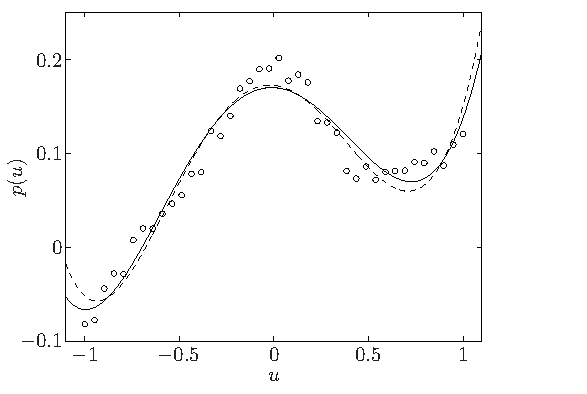
\includegraphics[width=.66\textwidth]{ch06-19.pdf}
\caption*{图6.19\quad 逼近图中以圆圈标出的40个数据点的两个5次多项式。实线多项式最小化误差的 $\ell_2$ 范数，虚线多项式最小化误差的 $\ell_\infty$ 范数。}
\end{figure}
\begin{figure}[htbp]\centering
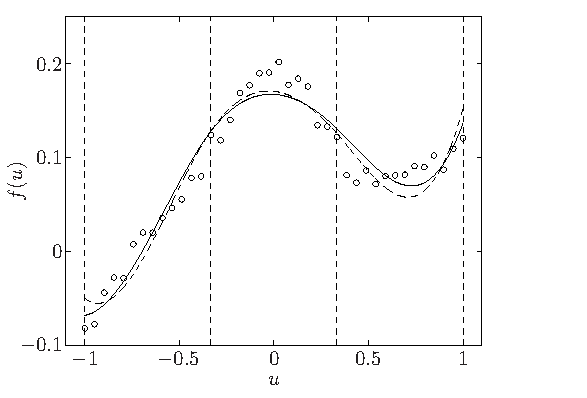
\includegraphics[width=.66\textwidth]{ch06-20.pdf}
\caption*{图6.20\quad 逼近图中以圆圈标出的40个数据点的两个三次样条；数据与图6.19相同。实线样条最小化误差的 $\ell_2$ 范数，虚线样条最小化误差的 $\ell_\infty$ 范数。与图6.19中的多项式逼近一样，拟合函数子空间的维数为6。}
\end{figure}

% Source PDF page 347 (printed p. 333)
\begin{origexample}{6.8}
\emph{样条拟合。}图6.20给出与例6.7相同的数据，以及用三次样条得到的两个最优拟合。将区间 $[-1,1]$ 等分为三个区间，考虑最高次数为3、一阶和二阶导数连续的分段多项式。这个函数子空间的维数为6，与例6.7中最高次数为5的多项式空间维数相同。
\end{origexample}

在最简单的函数拟合中，有 $m\gg n$，即数据点数远大于函数子空间维数。由于子空间中的所有函数都平滑，拟合会自动起到平滑作用。

\subsubsection*{最小范数插值}
在函数拟合的另一种变体中，数据点数少于函数子空间维数。最简单的情形，是要求选定函数满足插值条件
\[f(u_i)=y_i,\qquad i=1,\ldots,m,\]
这是关于 $x$ 的线性等式约束。在满足这些插值条件的函数中，可以寻找最平滑或最小的函数。这就得到最小范数问题。

在最一般的函数拟合问题中，可以在表示对背后函数的先验知识的各种凸约束下，优化某个目标，例如某种误差 $e$ 的度量。

\subsubsection*{插值、外推与求界}
在原数据集之外的点 $v$ 计算最优拟合函数 $\widehat f$，就得到对背后函数在 $v$ 处取值的猜测。如果 $v$ 位于给定数据点之间或附近，例如 $v\in\conv\{v_1,\ldots,v_m\}$，这称为\emph{插值}；否则称为\emph{外推}。

还可以在约束下最大化、最小化线性函数 $f(v)$，得到 $f(v)$ 可能取值的区间。可以利用函数拟合帮助识别错误数据或离群值。例如，采用 $\ell_1$ 范数拟合后，寻找误差较大的数据点。

\subsection{稀疏描述与基追踪}
在\emph{基追踪}中，基函数的数量非常大，目标是用少量基函数的线性组合很好地拟合给定数据。（此时函数族线性相关，有时称为\emph{过完备基}或\emph{字典}。）之所以称为基追踪，是因为要从给定过完备基中选出小得多的一组基来描述数据。

% Source PDF page 348 (printed p. 334)
因此，要寻找一个很好拟合数据的函数 $f\in\mathcal F$，使
\[f(u_i)\approx y_i,\qquad i=1,\ldots,m,\]
且系数向量 $x$ 稀疏，即 $\operatorname{card}(x)$ 小。此时称
\[f=x_1f_1+\cdots+x_nf_n=\sum_{i\in\mathcal B}x_if_i,\]
为数据的\emph{稀疏描述}，其中 $\mathcal B=\{i\mid x_i\ne0\}$ 是被选中基元素的指标集。从数学上看，基追踪与回归向量选择问题相同（见第6.4节），但优化问题的解释和规模不同。

稀疏描述与基追踪有许多用途，可以用于去噪、平滑，或对信号进行数据压缩以便高效传输或存储。在数据压缩中，发送方和接收方都知道字典或基元素。为了向接收方发送信号，发送方先寻找信号的稀疏表示，再只把非零系数以某种精度传给接收方。接收方用这些系数就能重构原信号的一个近似。

一种常用的基追踪方法，与第6.4节描述的回归向量选择方法相同，以 $\ell_1$ 范数正则化作为寻找稀疏描述的启发式方法。首先求解凸问题
\begin{equation}\text{最小化}\quad\sum_{i=1}^m(f(u_i)-y_i)^2+\gamma\norm x_1,\tag{6.18}\end{equation}
其中参数 $\gamma>0$ 用于在拟合数据的质量与系数向量的稀疏程度之间权衡。可以直接采用这个问题的解，也可以再进行精修：使用问题 (6.18) 的解所具有的稀疏模式，寻找最佳拟合。换言之，先求解 (6.18) 得到 $\widehat x$，然后令 $\mathcal B=\{i\mid\widehat x_i\ne0\}$，即非零系数对应的指标集。随后求解最小二乘问题
\[\text{最小化}\quad\sum_{i=1}^m(f(u_i)-y_i)^2,\]
变量为 $x_i$（$i\in\mathcal B$），并令 $i\notin\mathcal B$ 时 $x_i=0$。

基追踪与稀疏描述应用中的字典往往非常大，$n$ 可以在 $10^4$ 量级甚至更大。要高效求解 (6.18)，算法必须利用源于字典信号结构的问题结构。

\subsubsection*{用基追踪进行时频分析}
本节用一个简单例子说明基追踪与稀疏表示。考虑 $\R$ 上的函数或信号，关注范围为 $[0,1]$。把自变量理解为时间，因此用 $t$ 而非 $u$ 表示它。

先描述字典中的基函数。每个基函数都是一个高斯正弦脉冲，即 Gabor 函数，形式为
\[e^{-(t-\tau)^2/\sigma^2}\cos(\omega t+\phi),\]
其中 $\sigma>0$ 给出脉冲宽度，$\tau$ 是脉冲中心的时刻，$\omega\ge0$ 是频率，$\phi$ 是相位角。

% Source PDF page 349 (printed p. 335)
\begin{figure}[htbp]\centering
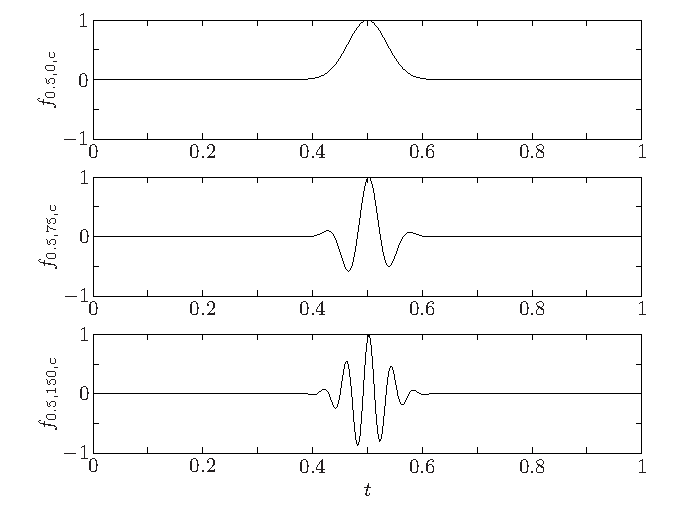
\includegraphics[width=.84\textwidth]{ch06-21.pdf}
\caption*{图6.21\quad 字典中的三个基元素，中心时刻均为 $\tau=0.5$，且均取余弦相位。上方信号频率为 $\omega=0$，中间为 $\omega=75$，下方为 $\omega=150$。}
\end{figure}
所有基函数宽度均为 $\sigma=0.05$。脉冲时刻与频率分别取
\[\tau=0.002k,\quad k=0,\ldots,500,\qquad\omega=5k,\quad k=0,\ldots,30.\]
对每个时刻 $\tau$，有一个零频率基元素（相位 $\phi=0$），以及其余30个频率各两个基元素（余弦和正弦，即相位 $\phi=0$、$\phi=\pi/2$），总共 $501\times61=30561$ 个基元素。自然可按时刻、频率与相位（余弦或正弦）对基元素编号，记作
\[\begin{aligned}
f_{\tau,\omega,c},&\quad\tau=0,0.002,\ldots,1,\quad\omega=0,5,\ldots,150,\\
f_{\tau,\omega,s},&\quad\tau=0,0.002,\ldots,1,\quad\omega=5,\ldots,150.
\end{aligned}\]
图6.21给出三个基函数，时刻均为 $\tau=0.5$。

采用这个字典的基追踪，可以看作对数据的时频分析。如果基元素 $f_{\tau,\omega,c}$ 或 $f_{\tau,\omega,s}$ 出现在信号的稀疏表示中，即对应系数非零，就可解释为：数据在时刻 $\tau$ 含有频率 $\omega$。

用基追踪寻找信号
\[y(t)=a(t)\sin\theta(t)\]
的稀疏近似，其中
\[a(t)=1+0.5\sin(11t),\qquad\theta(t)=30\sin(5t).\]

% Source PDF page 350 (printed p. 336)
\begin{figure}[htbp]\centering
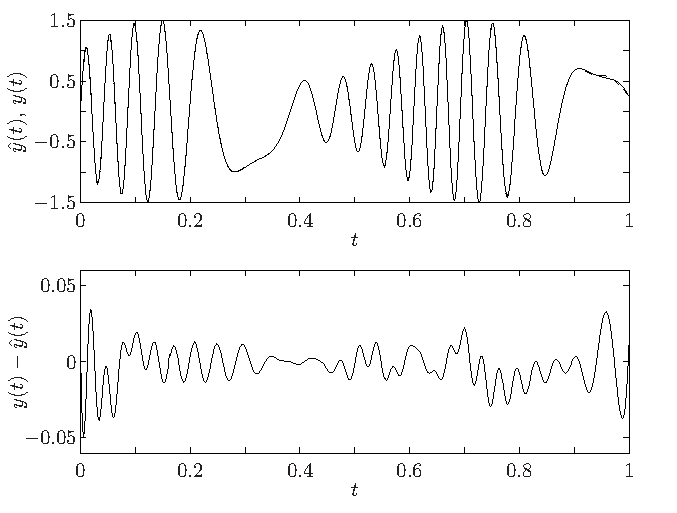
\includegraphics[width=.82\textwidth]{ch06-22.pdf}
\caption*{图6.22\quad 上：原信号（实线）与基追踪得到的近似 $\widehat y$（虚线）几乎无法区分。下：逼近误差 $y(t)-\widehat y(t)$，纵轴采用不同尺度。}
\end{figure}
（选择这个信号，仅仅因为它容易描述，而且其频谱成分随时间有明显变化。）可以将 $a(t)$ 理解为信号幅度，$\theta(t)$ 理解为总相位。还可以将
\[\omega(t)=\left|\frac{d\theta}{dt}\right|=150|\cos(5t)|\]
解释为信号在时刻 $t$ 的瞬时频率。数据为区间 $[0,1]$ 上501个均匀间隔采样，即501对数据 $(t_k,y_k)$，满足
\[t_k=0.005k,\qquad y_k=y(t_k),\qquad k=0,\ldots,500.\]

首先以 $\gamma=1$ 求解 $\ell_1$ 范数正则化最小二乘问题 (6.18)。所得最优系数向量非常稀疏，30561个系数中仅42个非零。然后用这42个基向量对原信号作最小二乘拟合。图6.22将结果 $\widehat y$ 与原信号 $y$ 作比较。上图中的近似信号（虚线）与原信号 $y(t)$（实线）几乎无法区分；下图给出误差 $y(t)-\widehat y(t)$。图中清楚表明，所得近似 $\widehat y$ 的相对拟合效果非常好。

% Source PDF page 351 (printed p. 337)
\begin{figure}[htbp]\centering
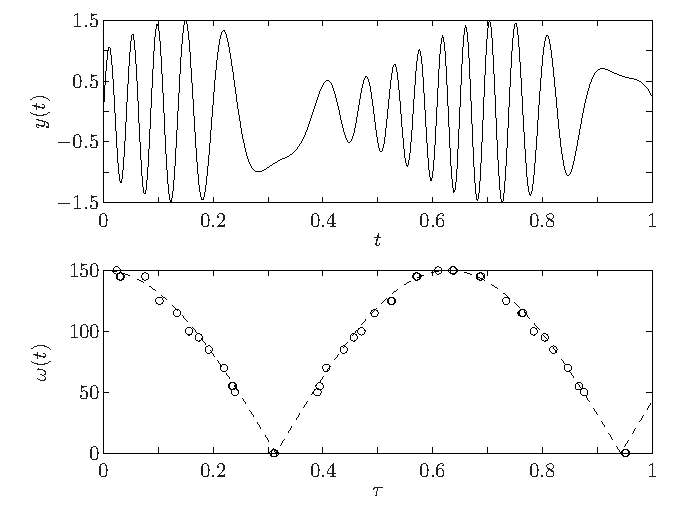
\includegraphics[width=.82\textwidth]{ch06-23.pdf}
\caption*{图6.23\quad 上：原信号。下：时频图。虚线表示原信号的瞬时频率 $\omega(t)=150|\cos(5t)|$。每个圆圈对应基追踪近似中选用的一个基元素，横轴为基元素的时刻指标 $\tau$，纵轴为频率指标 $\omega$。}
\end{figure}
相对误差为
\[\frac{(1/501)\sum_{i=1}^{501}(y(t_i)-\widehat y(t_i))^2}{(1/501)\sum_{i=1}^{501}y(t_i)^2}=2.6\cdot10^{-4}.\]

将非零系数的分布模式按时刻与频率绘出，就得到原始数据的时频分析。图6.23给出了这样的图，并同时绘出瞬时频率。图中可见，非零分量紧密跟随瞬时频率。

\subsection{用凸函数插值}
在一些特殊情形下，可以使用有限维凸优化，求解涉及无限维函数集合的插值问题。本节给出一个例子。

先问下面的问题：什么时候存在凸函数 $f:\R^k\to\R$，$\dom f=\R^k$，满足给定点 $u_i\in\R^k$ 上的插值条件
\[f(u_i)=y_i,\qquad i=1,\ldots,m?\]
（这里不要求 $f$ 位于任何有限维函数子空间中。）答案是：当且仅当存在 $g_1,\ldots,g_m$，使

% Source PDF page 352 (printed p. 338)
\begin{equation}y_j\ge y_i+g_i^\T(u_j-u_i),\qquad i,j=1,\ldots,m.\tag{6.19}\end{equation}
为证明这一点，先假设 $f$ 为凸函数，$\dom f=\R^k$，且 $f(u_i)=y_i$，$i=1,\ldots,m$。在每个 $u_i$ 处，都可找到向量 $g_i$，使对所有 $z$ 有
\begin{equation}f(z)\ge f(u_i)+g_i^\T(z-u_i).\tag{6.20}\end{equation}
如果 $f$ 可微，可取 $g_i=\nabla f(u_i)$；一般情况下，可以在 $(u_i,y_i)$ 处寻找 $\epi f$ 的一个支撑超平面来构造 $g_i$。（向量 $g_i$ 称为次梯度。）在 (6.20) 中取 $z=u_j$，即得到 (6.19)。

反之，假设 $g_1,\ldots,g_m$ 满足 (6.19)。对所有 $z\in\R^k$，定义
\[f(z)=\max_{i=1,\ldots,m}\bigl(y_i+g_i^\T(z-u_i)\bigr).\]
显然，$f$ 是分段线性的凸函数。不等式 (6.19) 蕴含 $f(u_i)=y_i$，$i=1,\ldots,m$。

利用这一结果，可以求解若干涉及用凸函数插值、逼近或求界的问题。

\subsubsection*{用凸函数拟合给定数据}
最简单的应用，也许是计算凸函数对给定数据 $(u_i,y_i)$（$i=1,\ldots,m$）的最小二乘拟合：
\[\begin{array}{ll}\text{最小化}&\displaystyle\sum_{i=1}^m(y_i-f(u_i))^2\\\text{约束条件}&f:\R^k\to\R\text{ 为凸函数},\quad\dom f=\R^k.\end{array}\]
这是一个无限维问题，因为变量 $f$ 位于 $\R^k$ 上的连续实值函数空间中。利用上述结果，可以将问题表述为
\[\begin{array}{ll}\text{最小化}&\displaystyle\sum_{i=1}^m(y_i-\widehat y_i)^2\\\text{约束条件}&\widehat y_j\ge\widehat y_i+g_i^\T(u_j-u_i),\quad i,j=1,\ldots,m,\end{array}\]
这是以 $\widehat y\in\R^m$ 和 $g_1,\ldots,g_m\in\R^k$ 为变量的 QP。当且仅当给定数据能由凸函数插值，即存在满足 $f(u_i)=y_i$ 的凸函数时，该问题最优值为零。图6.24给出一个例子。

\subsubsection*{对插值凸函数的取值求界}
另一个简单例子是：给定可由凸函数插值的数据 $(u_i,y_i)$，$i=1,\ldots,m$。对于另一个点 $u_0\in\R^k$，希望确定任意插值这些数据的凸函数 $f$ 的 $f(u_0)$ 可能取值范围。为求 $f(u_0)$ 的最小可能值，求解 LP
\[\begin{array}{ll}\text{最小化}&y_0\\\text{约束条件}&y_j\ge y_i+g_i^\T(u_j-u_i),\quad i,j=0,\ldots,m,\end{array}\]
变量为 $y_0\in\R$ 和 $g_0,\ldots,g_m\in\R^k$。将目标改为最大化 $y_0$（仍是 LP），就能找出插值给定数据的凸函数在 $u_0$ 处的最大可能值。

% Source PDF page 353 (printed p. 339)
\begin{figure}[htbp]\centering
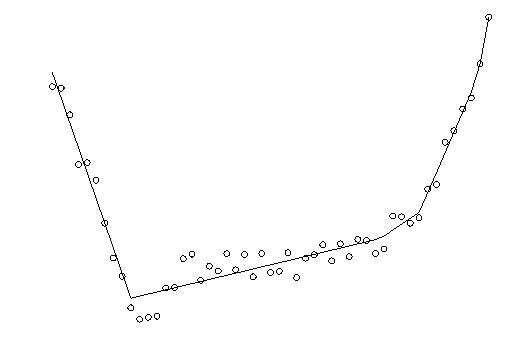
\includegraphics[width=.65\textwidth]{ch06-24.pdf}
\caption*{图6.24\quad 凸函数对以圆圈标出的数据的最小二乘拟合。图中的分段线性函数，在所有凸函数中使拟合误差的平方和最小。}
\end{figure}
\subsubsection*{用单调凸函数插值}
作为凸插值的扩展，可以考虑用凸且单调不减的函数插值。可以证明，存在凸函数 $f:\R^k\to\R$，$\dom f=\R^k$，满足插值条件
\[f(u_i)=y_i,\qquad i=1,\ldots,m,\]
且单调不减（$u\succeq v$ 时有 $f(u)\ge f(v)$），当且仅当存在 $g_1,\ldots,g_m\in\R^k$，使
\begin{equation}
\begin{gathered}
g_i\succeq0,\quad i=1,\ldots,m,\\
y_j\ge y_i+g_i^\T(u_j-u_i),\quad i,j=1,\ldots,m.
\end{gathered}\tag{6.21}
\end{equation}
也就是说，在凸插值条件 (6.19) 之外，再加上所有次梯度 $g_i$ 非负的条件。（见习题6.12。）

\subsubsection*{消费者偏好的推断与界定}
作为应用，考虑预测消费者偏好的问题。考虑由 $n$ 种消费品的不同数量组成的商品篮子。一个商品篮子用向量 $x\in[0,1]^n$ 表示，其中 $x_i$ 是第 $i$ 种商品的数量。假设数量已经归一化，使 $0\le x_i\le1$，其中 $x_i=0$、$x_i=1$ 分别是商品 $i$ 的最少与最多可能数量。给定两个商品篮子 $x$、$\widetilde x$，消费者可能更喜欢 $x$，可能更喜欢 $\widetilde x$，也可能认为两者同样有吸引力。考虑一位选择具有可重复性的模型消费者。

% Source PDF page 354 (printed p. 340)
按以下方式刻画消费者偏好。假设存在效用函数 $u:\R^n\to\R$，定义域为 $[0,1]^n$；$u(x)$ 衡量消费者从商品篮子 $x$ 中获得的效用。面对两个商品篮子，消费者选择效用较大的一个；如果两者效用相等，就无所谓选择哪一个。合理的假设是 $u$ 单调不减，这表示在其他商品数量保持不变时，消费者总希望任意一种商品更多一些。同样合理的是假设 $u$ 为凹函数，它刻画随着商品数量增加而出现的满足效应，即边际效用递减。

现在，假设给定一些消费者偏好数据，但不知道背后的效用函数 $u$。具体地，给定商品篮子集合 $a_1,\ldots,a_m\in[0,1]^n$，以及它们之间的一些偏好信息：
\begin{equation}
u(a_i)>u(a_j)\quad((i,j)\in\mathcal P),\qquad
u(a_i)\ge u(a_j)\quad((i,j)\in\mathcal P_{\rm weak}),\tag{6.22}
\end{equation}
其中 $\mathcal P,\mathcal P_{\rm weak}\subseteq\{1,\ldots,m\}\times\{1,\ldots,m\}$ 已知。$\mathcal P$ 给出已知严格偏好的集合：$(i,j)\in\mathcal P$ 表示已知消费者更喜欢篮子 $a_i$ 而非 $a_j$。集合 $\mathcal P_{\rm weak}$ 给出已知弱偏好：$(i,j)\in\mathcal P_{\rm weak}$ 表示 $a_i$ 比 $a_j$ 更受偏好，或者两者同样有吸引力。

先考虑如何判断数据是否一致，即是否存在满足 (6.22) 的凹且不减的效用函数 $u$。这等价于求解可行性问题
\begin{equation}
\begin{array}{ll}\text{寻找}&u\\\text{约束条件}&u:\R^n\to\R\text{ 为凹且不减的函数},\\&u(a_i)>u(a_j),\quad(i,j)\in\mathcal P,\\&u(a_i)\ge u(a_j),\quad(i,j)\in\mathcal P_{\rm weak},\end{array}\tag{6.23}
\end{equation}
以函数 $u$ 作为无限维优化变量。由于 (6.23) 中所有约束都是齐次的，可以将问题等价地写为
\begin{equation}
\begin{array}{ll}\text{寻找}&u\\\text{约束条件}&u:\R^n\to\R\text{ 为凹且不减的函数},\\&u(a_i)\ge u(a_j)+1,\quad(i,j)\in\mathcal P,\\&u(a_i)\ge u(a_j),\quad(i,j)\in\mathcal P_{\rm weak},\end{array}\tag{6.24}
\end{equation}
只使用非严格不等式。（显然，满足 (6.24) 的 $u$ 必满足 (6.23)；反之，若 $u$ 满足 (6.23)，则可将其缩放以满足 (6.24)。）再利用第339页的插值结果，可将该问题写成有限维线性规划可行性问题：
\begin{equation}
\begin{array}{ll}\text{寻找}&u_1,\ldots,u_m,g_1,\ldots,g_m\\\text{约束条件}&g_i\succeq0,\quad i=1,\ldots,m,\\&u_j\le u_i+g_i^\T(a_j-a_i),\quad i,j=1,\ldots,m,\\&u_i\ge u_j+1,\quad(i,j)\in\mathcal P,\\&u_i\ge u_j,\quad(i,j)\in\mathcal P_{\rm weak}.\end{array}\tag{6.25}
\end{equation}
求解这个线性规划可行性问题，就能确定是否存在与给定严格和非严格偏好集合一致的凹且不减的效用函数。
